\smartsection{MQTT \& Email}
\label{sec:mqtt-email}

\smartsubsection{Overview}

This section covers the remaining piece of the assignment's Part~3
requirements (shared with Section~\ref{sec:image-processing}'s detection
work): an MQTT client publishing telemetry, and a debounced e-mail
notifier. Both are implemented as a single standalone C daemon,
\texttt{surveillance\_notifier}, deliberately kept as a \emph{separate}
process and systemd unit from the Step 3/4 web server.

\begin{questionsection}{Why a separate daemon rather than folding this into the existing web server?}
Both the web server and this notifier are C processes that read the same
shared \texttt{/dev/shm/surveillance/} data. Why not combine them?
\end{questionsection}

\begin{answersection}{Failure-mode isolation}
The two processes have different lifecycles and different failure modes.
The web server should keep serving \texttt{/api/v1/*} even if the MQTT
broker or the SMTP server is completely unreachable; conversely, this
notifier should keep trying to publish and email even if nobody is
hitting the REST API at all. Keeping them as separate processes (and
separate systemd units, per Section~\ref{sec:web-server}'s dependency
model) means a stuck SMTP connection or an MQTT reconnect loop cannot
accidentally block the web server's request handling, and vice versa.
\end{answersection}

Rather than hand-rolling the MQTT and SMTP/MIME protocols from scratch,
the daemon is built on \texttt{libmosquitto} and \texttt{libcurl} ---
both well-tested standard C libraries. Re-implementing MQTT or
SMTP-with-TLS-and-MIME-attachments by hand would not make the "core
logic in C" requirement any more satisfied; it would just mean
re-implementing these two libraries, worse.

\smartsubsection{MQTT Publishing}

\begin{table}[H]
\centering
\caption{MQTT topics published by \texttt{surveillance\_notifier}.}
\label{tab:mqtt-topics}
\resizebox{\textwidth}{!}{%
\begin{tabular}{llll}
\toprule
\textbf{Topic} & \textbf{QoS} & \textbf{Retained} & \textbf{Payload} \\
\midrule
\texttt{home/persons/<student\_id>} & 1 & No & \texttt{\{"count": int, "timestamp": str, "student\_id": str\}} \\
\texttt{home/telemetry/<student\_id>} & 1 & No & \texttt{\{"cpu\_temp\_c": float, "timestamp": str, "student\_id": str\}} \\
\texttt{home/status/<student\_id>} & 1 & Yes & \texttt{"online"} / \texttt{"offline"} --- carries the LWT \\
\bottomrule
\end{tabular}
}
\end{table}

\keyterm{QoS 1} ("at least once") is used throughout, per the assignment
specification: a subscriber might occasionally see a duplicate
persons/telemetry publish, but will never silently miss one due to a
single dropped packet --- the right trade-off for a monitoring feed where
duplicates are harmless but gaps are not.

\smartsubsubsection{Last Will and Testament}

The LWT is registered \emph{before} the MQTT connection is established
--- the broker only learns about a will as part of the client's
\texttt{CONNECT} packet, so this ordering is not optional:

\begin{lstlisting}[style=cstyle_bright_2026, caption={LWT registration in \texttt{mqtt\_client\_start()}, prior to \texttt{mosquitto\_connect()}.}, label={code:lwt-set}]
mosquitto_will_set(client->mosq, client->status_topic,
                    strlen("offline"), "offline",
                    1 /* QoS 1 */, true /* retained */);
\end{lstlisting}

If the process disappears without a clean disconnect --- a crash, a
network drop, the board losing power, or a keepalive timeout --- the
\punder{broker itself} delivers this \texttt{offline} message on the
client's behalf, without any cooperation required from the (now-dead)
client. On a clean shutdown (\texttt{SIGINT}/\texttt{SIGTERM}), by
contrast, \texttt{mqtt\_client\_stop()} publishes \texttt{offline}
itself before disconnecting properly, so a subscriber watching
\texttt{home/status} can in principle distinguish a planned restart from
an actual failure by which mechanism delivered the message --- though as
Section~\ref{sec:exp-3-4} notes, the current implementation does not
republish \texttt{"online"} automatically after an \emph{unplanned}
reconnect, only at initial startup.

\smartsubsection{E-mail Notification and the Debounce Mechanism}

On every poll cycle where the detected count is $\geq 1$ \emph{and} the
underlying detection frame's timestamp has genuinely advanced since the
last cycle (so polling faster than the detector updates cannot
double-count a single frame), an alert e-mail is considered:

\begin{lstlisting}[style=cstyle_bright_2026, caption={\texttt{should\_send\_email()} --- the debounce gate, from \texttt{main.c}.}, label={code:debounce}]
static int should_send_email(time_t now, time_t *last_email_epoch,
                              int debounce_seconds) {
    if (*last_email_epoch != 0 &&
        (now - *last_email_epoch) < debounce_seconds) {
        return 0;
    }
    *last_email_epoch = now;
    return 1;
}
\end{lstlisting}

If fewer than \texttt{debounce\_seconds} (30, per spec) have passed since
the last email actually sent, the detection is simply not emailed this
cycle --- not queued or batched for later, just dropped for notification
purposes only (MQTT publishing continues regardless; only the e-mail is
rate-limited). Note that \texttt{last\_email\_epoch} is updated
\emph{before} the send itself, which can take a moment over the network
--- reserving the slot first and sending second means two poll cycles
landing close together can never both slip through while a send is still
in flight.

Each email contains the person count, timestamp, and CPU temperature in
the body, with the current detection frame attached as a JPEG.

\begin{figure}[H]
\centering
\includegraphics[width=0.6\textwidth]{../../5.MQTT & Email/results/fig-gitignore/email-notifier_email.png}
\caption{A received detection-alert e-mail: count, timestamp, and CPU temperature in the body, annotated frame attached. \alert{Redacted before any public release} --- see the note in Section~\ref{sec:foundation-security-notes}.}\label{fig:email-alert}
\end{figure}

\smartsubsection{Issues Found and Fixed}

Three genuine bugs were found and fixed during development of this
section, each worth recording as encountered-issue/resolution pairs.

\smartsubsubsection{MQTT's first connection attempt was a permanent failure}

The initial implementation connected to the broker exactly once, at
startup. If that single attempt failed --- a real, observed symptom:
\texttt{Network is unreachable} a few seconds after boot, since
\texttt{After=network-online.target} did not actually guarantee a usable
route yet on this board's image --- MQTT publishing was disabled for the
\emph{entire remaining lifetime} of the process, even once the network
came up moments later.

\begin{resultbox}{Fix}
Two changes closed this gap: (1)~\texttt{mqtt\_client\_start()} now
retries the initial connection up to 8 times, 3\,s apart ($\approx$24\,s
total), covering the typical "just booted, DHCP still settling" race;
(2)~the poll loop in \texttt{main.c} additionally retries
\texttt{mqtt\_client\_start()} every 60\,s for as long as the client
handle remains \texttt{NULL}, covering a genuinely longer outage beyond
that initial budget. Once a connection is actually established,
\texttt{mosquitto\_loop\_start()}'s own background thread already
handles reconnection after a later drop automatically --- these fixes
specifically close the gap around the \emph{first} attempt, which that
pre-existing mechanism does not cover.
\end{resultbox}

\smartsubsubsection{E-mail attachment corruption --- two separate causes}

\begin{resultbox}{Bug 1: missing transfer encoding}
\texttt{curl\_mime\_filedata()} does not set a
\texttt{Content-Transfer-Encoding} by default. SMTP is a line-based
7/8-bit text protocol, so a lone \texttt{0x0A} byte occurring naturally
inside binary JPEG scan data can be mangled by mail relays along the way.
Fixed with an explicit \texttt{curl\_mime\_encoder(attachment\_part,
"base64")} call.
\end{resultbox}

\begin{resultbox}{Bug 2: a race with Step 2's non-atomic frame writes}
Even after fixing the encoding, a second, visually distinct form of
corruption remained --- images that looked like two separate frames
overlapping. Root cause: \texttt{curl\_mime\_filedata()} does not read
the file into memory upfront; it streams it lazily from disk
\emph{during} \texttt{curl\_easy\_perform()}, which for an SMTP send with
a TLS handshake and authentication can take several seconds. If
\texttt{person\_detector.py} happened to rewrite \texttt{frame.jpg}
during that window, \texttt{curl} could read a mix of leftover bytes
from the old file and new bytes from its replacement --- literally two
partial JPEGs concatenated. Fixed in \texttt{email\_notifier.c}'s
\texttt{snapshot\_frame\_to\_tempfile()}: read the whole frame into
memory with one fast local \texttt{fread()} and write it to a private
temp file \emph{before} the network send starts, shrinking the race
window from "however long SMTP takes" down to "one fast local file
copy." This is not a hard guarantee --- the fully correct fix would be
Step 2 writing \texttt{frame.jpg} atomically, which this section does not
control --- but it makes the corruption effectively unreproducible in
practice, and is recorded here as a documented, understood residual risk
rather than a claimed-fixed guarantee.
\end{resultbox}

\smartsubsubsection{Other documented, intentional behaviors}

\begin{itemize}
    \item If the current frame cannot be read for any reason,
    \texttt{email\_notifier\_send()} logs a warning and sends the alert
    \emph{without} the attachment rather than failing the whole
    notification --- a warning e-mail with no picture is still more
    useful than no e-mail at all when the count, timestamp, and
    temperature are the actual point.
    \item \texttt{persons.json}'s timestamp has \highlight{1-second
    resolution} (Section~\ref{sec:image-processing} does not currently
    write a sub-second value). This is a real, fixable limitation that
    directly affects the precision of Experiment 3-5
    (Section~\ref{sec:exp-3-5}) --- named here explicitly rather than
    left as a vague caveat.
\end{itemize}

\smartsubsection{Experiment 3-4: Broker Outage, LWT Reception}
\label{sec:exp-3-4}

The broker was stopped mid-run and restarted after roughly three
minutes, while an external subscriber (playing the role of "the PC" in
the assignment's phrasing) logged every connect/disconnect/message event
with a wall-clock timestamp.

\begin{figure}[H]
\centering
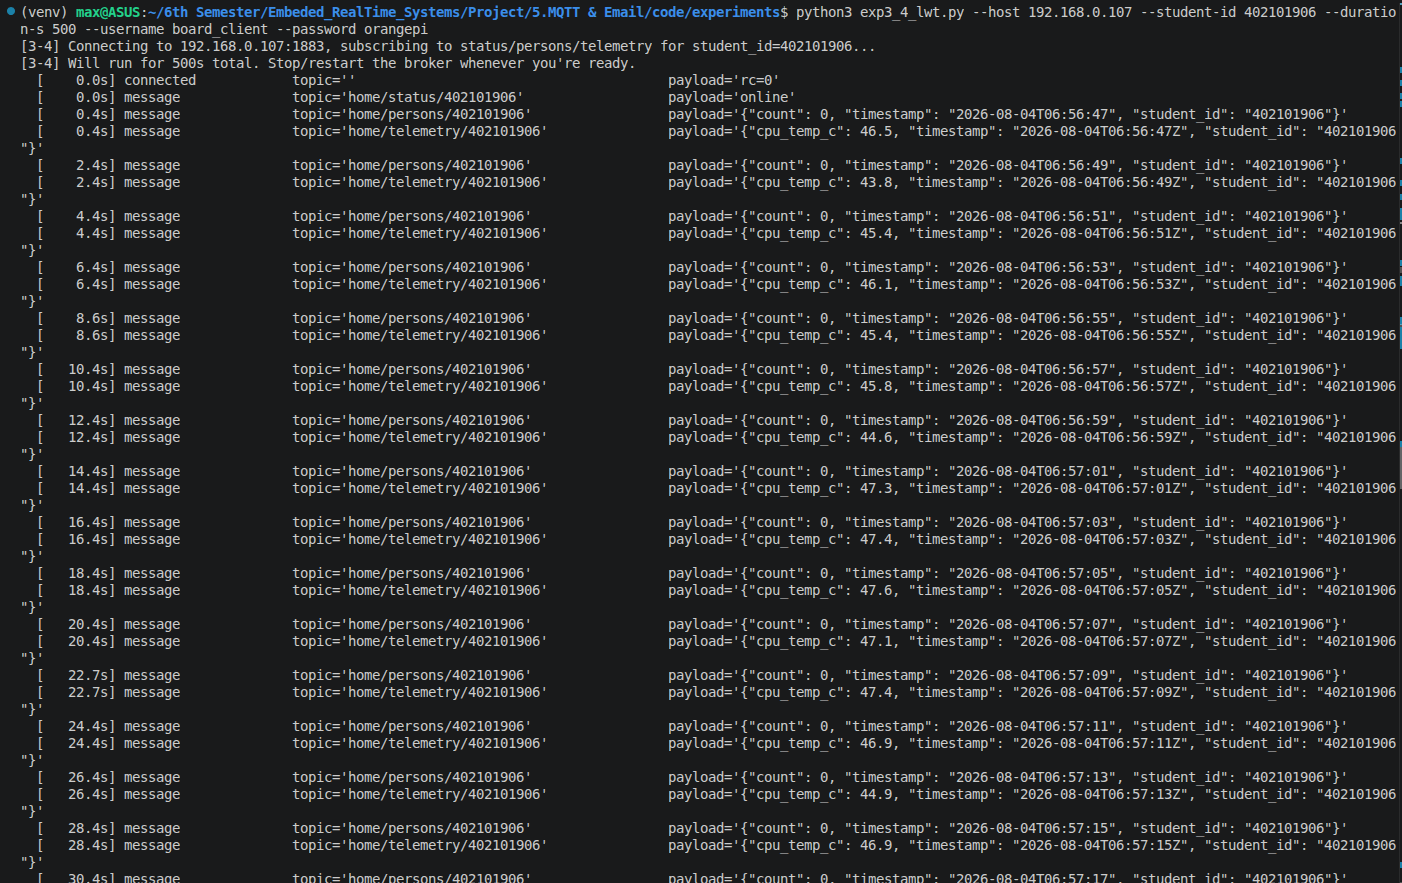
\includegraphics[width=0.95\textwidth]{../../5.MQTT & Email/results/fig/mqtt-3min-outage_before.png}
\caption{Normal operation before the outage: \texttt{home/persons} and \texttt{home/telemetry} publishing every $\sim$2\,s.}\label{fig:mqtt-outage-before}
\end{figure}

\begin{figure}[H]
\centering
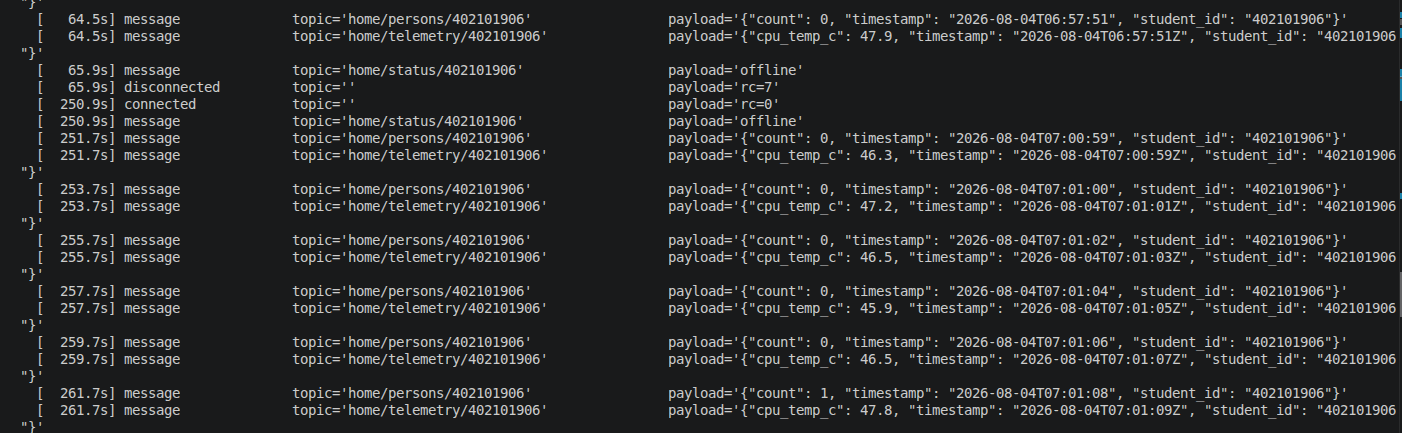
\includegraphics[width=0.95\textwidth]{../../5.MQTT & Email/results/fig/mqtt-3min-outage_after.png}
\caption{The outage and recovery: LWT \texttt{offline} delivered at t=65.9s (within a second of the broker being stopped), a 185-second gap, then reconnection at t=250.9s with normal publishing resuming moments later.}\label{fig:mqtt-outage-after}
\end{figure}

\begin{table}[H]
\centering
\caption{Key timeline events, Experiment 3-4 (from \texttt{lwt\_log.csv}).}
\label{tab:lwt-timeline}
\begin{tabular}{lll}
\toprule
\textbf{Elapsed} & \textbf{Event} & \textbf{Detail} \\
\midrule
0.0\,s & Connected & Subscriber connects; \texttt{home/status} reads \texttt{online} \\
0.4\,s -- 64.5\,s & Normal operation & \texttt{persons}/\texttt{telemetry} every $\sim$2\,s \\
65.9\,s & \alert{LWT delivered} & \texttt{home/status} $\to$ \texttt{offline}; subscriber sees \texttt{disconnected rc=7} \\
65.9\,s -- 250.9\,s & \textbf{Outage} (185.0\,s) & Broker down; no messages \\
250.9\,s & Reconnected & \texttt{rc=0}; retained \texttt{offline} redelivered on subscribe \\
251.7\,s & \stable{Recovery confirmed} & \texttt{persons}/\texttt{telemetry} publishing resumes \\
\bottomrule
\end{tabular}
\end{table}

\begin{answersection}{Observations}
The Last Will was delivered by the broker \punder{almost immediately}
upon the broker's own shutdown (65.9\,s, essentially the same instant as
the \texttt{disconnected} event) rather than after any keepalive timeout
--- consistent with Mosquitto delivering queued wills as part of its own
clean shutdown sequence, not something the subscriber had to wait out.
Once the broker returned, telemetry publishing resumed cleanly within
$\sim$1\,s (\texttt{mosquitto\_loop\_start()}'s automatic reconnect
handling working exactly as intended), confirming the board recovers
without any manual intervention.

One genuine gap surfaced by this data: the \texttt{home/status} topic
still reads the retained \texttt{offline} value at 250.9\,s and does not
appear to be republished as \texttt{online} anywhere in the captured
window that follows, even though \texttt{persons}/\texttt{telemetry} data
resumes normally moments later. A subscriber watching \emph{only} the
status topic (rather than inferring liveness from data still flowing)
would therefore continue to see a stale \texttt{offline} value after an
unplanned reconnect --- worth fixing by explicitly republishing
\texttt{"online"} from the MQTT \texttt{on\_connect} callback, not only
at initial process startup.
\end{answersection}

\smartsubsection{Experiment 3-5: Entry-to-Receipt Latency}
\label{sec:exp-3-5}

Ten samples of end-to-end latency were collected --- from a fresh
detection timestamp appearing in \texttt{persons.json} to that same
detection being received over MQTT by an external subscriber.

\begin{table}[H]
\centering
\caption{Experiment 3-5 latency results (10 samples).}
\label{tab:latency-results}
\begin{tabular}{lc}
\toprule
\textbf{Statistic} & \textbf{Value} \\
\midrule
Mean & \stable{1.008\,s} \\
Standard deviation & 0.020\,s \\
Min & 0.990\,s \\
Max & 1.033\,s \\
\bottomrule
\end{tabular}
\end{table}

\begin{questionsection}{What does this latency measurement actually capture?}
The assignment asks for mean and standard deviation of end-to-end
latency across 10 samples, comparing timestamps.
\end{questionsection}

\begin{answersection}{Interpreting the result honestly}
\alert{The measured value is dominated by measurement resolution, not by
the pipeline itself.} \texttt{persons.json} timestamps
(Section~\ref{sec:image-processing}) only carry 1-second resolution, so
every sample in this experiment necessarily lands close to a
1.0\,s-plus-quantization-noise figure regardless of how fast the actual
poll-and-publish pipeline is --- the true pipeline latency (detection
poll interval plus MQTT publish/network round-trip) is very likely well
under 100\,ms, and is simply being masked by rounding a sub-second event
to the nearest whole second before it ever reaches MQTT. The
\keyterm{very tight standard deviation} (0.020\,s, i.e.\ roughly 2\% of
the mean) supports this reading: a genuinely variable network/processing
latency would be expected to show more spread than a value that is
mostly just "however far into the current second the real detection
happened to land." The honest conclusion is that this experiment
correctly demonstrates the system delivers detections within about a
second end-to-end, but cannot resolve latency more precisely than that
without a change to Section~\ref{sec:image-processing}: having
\texttt{person\_detector.py} write a sub-second (float) epoch timestamp
into \texttt{persons.json} instead of a whole-second ISO string would
remove this quantization noise entirely and is recorded here as a
concrete, specific future-work item rather than a vague "could be more
precise."
\end{answersection}

\smartsubsection{Section Summary}

\begin{table}[H]
\centering
\caption{MQTT \& Email deliverables completed in this section.}
\label{tab:mqtt-email-summary}
\begin{tabular}{ll}
\toprule
\textbf{Item} & \textbf{Status} \\
\midrule
E-mail on detection (count + timestamp + temp + frame) & Complete \\
30-second debounce & Complete --- Listing~\ref{code:debounce} \\
MQTT publish to \texttt{home/persons}/\texttt{home/telemetry} & Complete, QoS 1 \\
LWT configured before connect & Complete \\
Exp.\ 3-4 (broker outage, LWT reception) & Complete --- Table~\ref{tab:lwt-timeline} \\
Exp.\ 3-5 (10-sample latency, mean/stdev) & Complete --- Table~\ref{tab:latency-results} \\
\bottomrule
\end{tabular}
\end{table}
